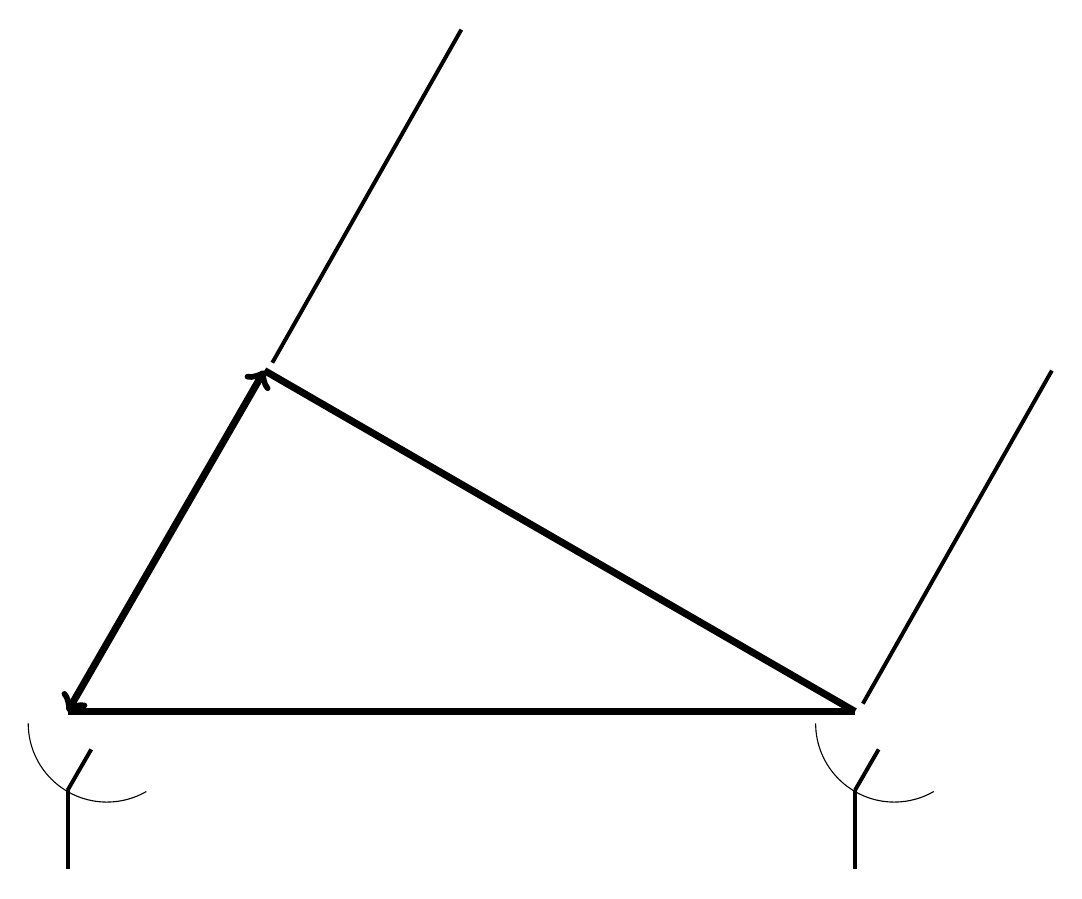
\begin{tikzpicture}

  % (* (sqrt (- (* 10 10) (* 5 5))) (cos (asin (/ 5.0 10.0))))7.5
  \draw[line width= 0.5mm, black]      ( 2.500*2,     4.330*2) -- ( 2.500+0.1,    4.330+0.1);
  \draw[line width= 0.5mm, black]      ( 2.500*2+7.5, 4.330  ) -- ( 2.500+0.1+7.5,      0.1);

  % (* 5 (sin (- (/ pi 2) (asin (/ 5.0 10.0))))) 4.330
  % (* 5 (cos (- (/ pi 2) (asin (/ 5.0 10.0))))) 2.500
  \draw[line width= 0.9mm, black]      (10.000, 0.000) -- (2.500, 4.330);
  \draw[line width= 0.9mm, black, <->] ( 2.500, 4.330) -- (0.000, 0.000);
  \draw[line width= 0.9mm, black]      (10.000, 0.000) -- (0.000, 0.000);

  \draw (  0-0.5, 0-0.15) arc (180:300:1cm);
  \draw ( 10-0.5, 0-0.15) arc (180:300:1cm);

  \draw[line width= 0.5mm, black] (10.0, -2.0) -- (10.0, -1.0);
  \draw[line width= 0.5mm, black] ( 0.0, -2.0) -- ( 0.0, -1.0);

  \draw[line width= 0.5mm, black] ( 2.500*1.12-2.5,     4.330*1.12-4.330-1) -- ( 2.500-2.5,    4.330-4.330-1);
  \draw[line width= 0.5mm, black] ( 2.500*1.12-2.5+10,     4.330*1.12-4.330-1) -- ( 2.500-2.5+10,    4.330-4.330-1);

\end{tikzpicture}

%%% Local Variables:
%%% mode: latex
%%% TeX-master: "../Lecture"
%%% End: